\newpage
\part{Bandits-manchots}

\section{Description du probl\`eme}
On condi\`ere le probl\`eme d'apprentissage suivant : un agent est confront\'e \`a plusieurs reprises \`a un choix parmi N diff\'erentes actions, chacune des N actions procure une r\'ecompense moyenne $\mu^{i}$ inconnue par l'agent et nous d\'esignons l'action sélectionnée sur le pas de temps t par $a_{t}$, la r\'ecompense correspondante par $r_{t}$ et $N_{T}(a)$ le nombre de fois o\‘u l’action $a$ a \'et\'e choisi jusqu'au temps T.  L'objectif est de maximiser la somme des r\'ecompense obtenue au bout des $T$ premi\‘eres parties, pour cel\`a, l'agent doit identifier l'action au rendement le plus elev\'e $i^{*}$= $\argmax_{i \in {1,\ldots,N}}\mu^{i}$. Les valeurs $\mu^{i}$ etant inconnues, il est donc necessaire de faire des estimations qui doivent  \^etre le plus repr\'esentatives possible des valeurs $\mu^{i}$, notons $\hat{\mu}^{i}$ ces estimations. L'estimation associ\'ee \‘a une action est la r\'ecompense moyenne lorsque cette action est s\'electionn\'ee.
\begin{equation*}
\hat{\mu}^{i} = \frac{1}{N_{T}(a)}\sum_{t=1}^{T} r_{t}\mathbbm{1}_{a_{t} = a}
\end{equation*}

\section{Algorithmes}
Si de nombreux algorithmes ont \'et\'e propos\'es pour r\'esoudre ce dilemme, on se contentera ici d'en citer que quelques uns:
\subsection{Algorithme Al\'eatoire}
l'algorithme al\'eatoire se contente de choisir l’action uniform\'ement au hasard. On peut donc d\'ej\`a pr\'esager que cet algorithme sera forc\'ement le moins optimal.
{\bfseries En effet, il effectue purement de l'exploitation et est ainsi utilis\'e comme baseline pour les tests pr\'esent\'es par la suite}
\subsection{Algorithme Greedy}
L'algorithme Greedy est bas\'e sur une politique de selection tr\`es simple qui consiste \`a s\'electionner l'une des actions ayant la valeur estim\'ee la plus \'elev\'ee :
$a_{t}$ = $\argmax_{i \in {1,\ldots,N}}\hat{\mu}^{i}_{t}$.
Autrement dit, L'algorithme Greedy ne fait qu'\'exploiter les connaissances dont on dispose afin de maximiser la recompense \`a un instant $t$.
\subsection{Algorithme $\varepsilon$-Greedy}
Une approche courante pour trouver un compromis exploitation/exploration est l'algorithme $\varepsilon$-Greedy qui consiste \‘a choisir \‘a l’instant $t$, avec une probabilit\'e 1 - $\varepsilon$, l’action qui maximise le rendement moyen sur les estimations faites jusque l\‘a et avec une probabilit\‘e $\varepsilon$, une action uniform\‘ement au hasard. L'avantage de cet algorithme repose sur le fait que dans la mesure o\`u le nombre d'étape d'apprentissage augmente, chaque action sera choisie un nombre infini de fois assurant ainsi que tous les $\hat{\mu}^{i}$ convergeront vers les $\mu^{i}$. On peut conj\'ecturer la puissance de cet algorithme et sa capacit\'e \‘a explorer toutes les actions possibles et de prendre des d\'ecisions quasi proches de l’optimum.
{\bfseries Je sais pas si c'est vraiment un nombre infini, mais c'est s\^ur que les estimateurs se rapprocheront davantage aux gains moyens r\'eels. On pourra aussi dire que la valeur de $\varepsilon$ a un fort impact sur l'apprentissage, c'est pourquoi on en a test\'e diff\'erentes valeurs (constantes) et m\^eme une forme en fonction (d\'ecroissante) du temps ???}

\subsection{Algorithme UCB}
L'algorithme UCB est une autre strat\'egie qui permet de trouver une balance entre l'exploration et l'exploitation. L'id\'ee de cet algorithme consiste \`a se fier \`a une borne sup\'erieure de confiance, en effet, une incertitude existera toujours sur l'optimalit\'e des estimations faites jusque l\`a. Les deux algorithmes d\'efinis pr\'ecedemment choisissent toujours l'action qui semble meileure \`a un instant $t$ ou se contentent de choisir des actions al\'eatoirement sans distinction. L'algorithme UCB prend en compte l'optimalit\'e des estimations mais egalement l'incertitude sur celles-ci. Il selectionne l'action : $a_{t}$ = $\argmax_{i \in {1,\ldots,N}}(\hat{\mu}^{i}_{t} + \sqrt{\frac{2\log(t)}{N_{T}(i)}})$.
{\bfseries Ici, cette incertitude est mesur\'ee par le deuxi\`eme terme : plus grand est le d\'es\'equilibre entre le(s) (nombre d') actions effectu\'ees, plus on se m\'efie au r\'esultats. On privili\'egiera ainsi les actions le plus d\'efavoris\'ees}
\newpage
\section{Mise en oeuvre et expérimentations}
\begin{figure}[htbp]
    \centering
    \begin{subfigure}[b]{0.47\textwidth} % "0.45" donne ici la largeur de l'image
        \centering 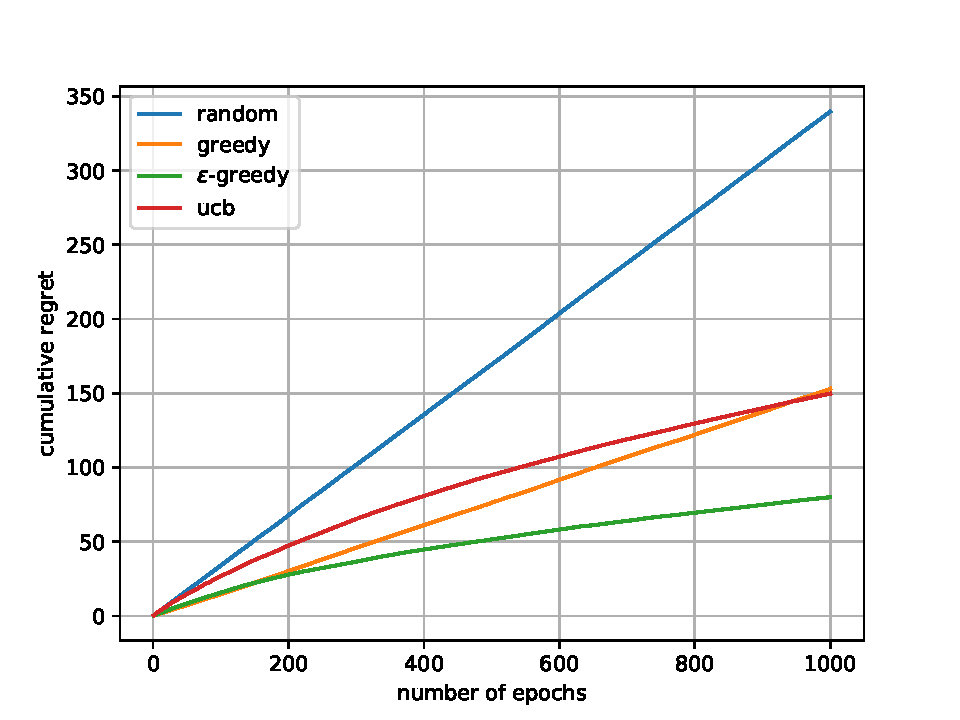
\includegraphics[width=\textwidth]{Report/sections/Figures/Figure1.pdf}
        \caption{Regret cumulé en fonction du nombre d'étape d'apprentissage}
    \end{subfigure}
    ~ 
    \begin{subfigure}[b]{0.47\textwidth}
        \centering 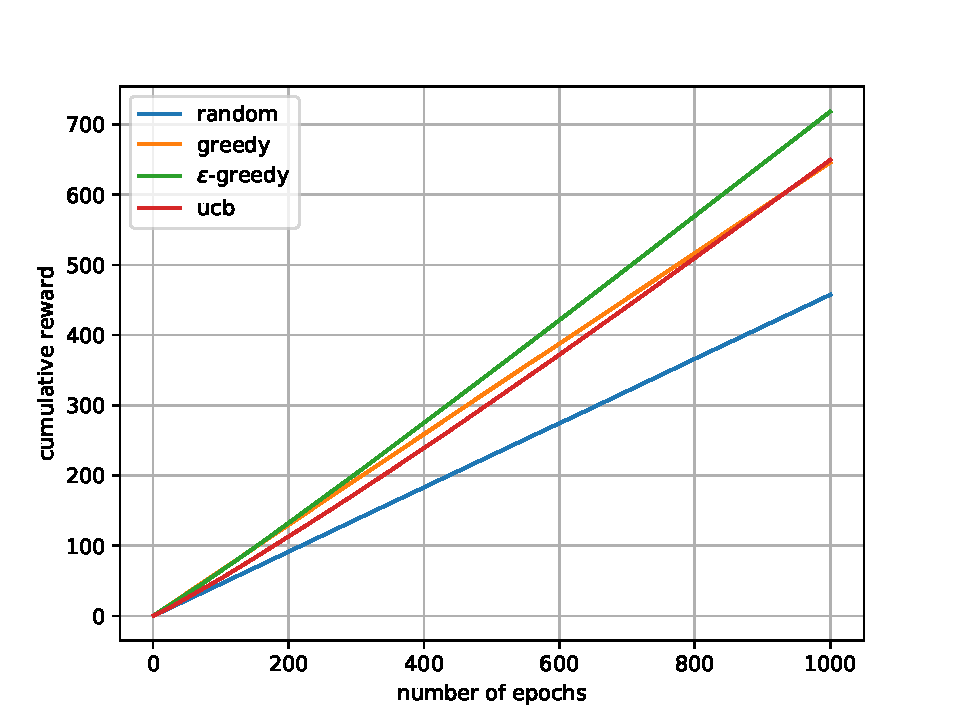
\includegraphics[width=\textwidth]{Report/sections/Figures/Figure2.pdf}
        \caption{Recompenses cumulés en fonction du nombre d'étape d'apprentissage}
    \end{subfigure}
    \caption{Performance des quatres algorithmes sur 10 leviers et en moyennant les résultats sur 400 éxecutions.}
\end{figure}
La figure 1 montre le gain et le regret cumulé en fonction de $t$ pour les quatre algorithmes décrits dans la section précédente. Nous avons fait le choix de simuler avec une machine à 10 léviers, chacun suit une loi de Bernoulli avec un paramètre choisi uniformément dans [0,1].
TODO : commenter les courbes ci-dessus. Il me semble qu'on est sensé remarquer une amelioration si on change la distribution de gain. En effet, si on a des gains qui suivent une distribution normale plutot qu'une distribution uniforme aléatoire, on remarquera une legere amelioration des performance pour chaque algorithme. Cela est logique, car l'action optimale est mieux "s"paré" des autres actions (ici il serait plus judicieux de favoriser l'exploitation plutot que l'exploration)

\begin{figure}[htbp]
   \begin{subfigure}[b]{0.47\textwidth}
        \centering 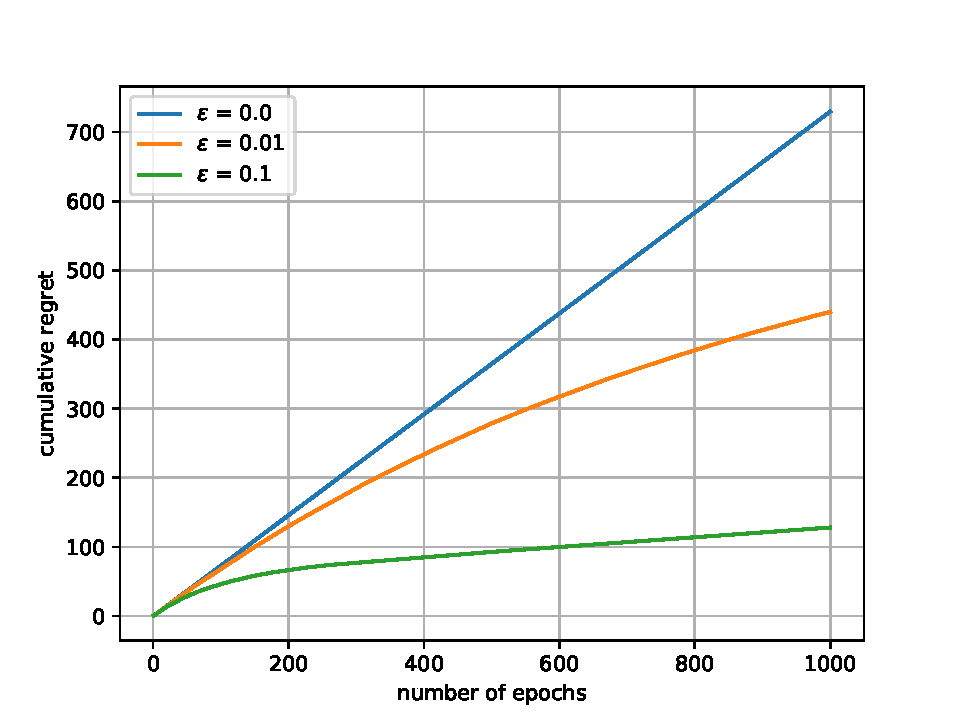
\includegraphics[width=\textwidth]{Report/sections/Figures/Figure3.pdf}
        \caption{Regret cumulé en fonction du nombre d'étape d'apprentissage}
    \end{subfigure}
    \begin{subfigure}[b]{0.47\textwidth}
        \centering 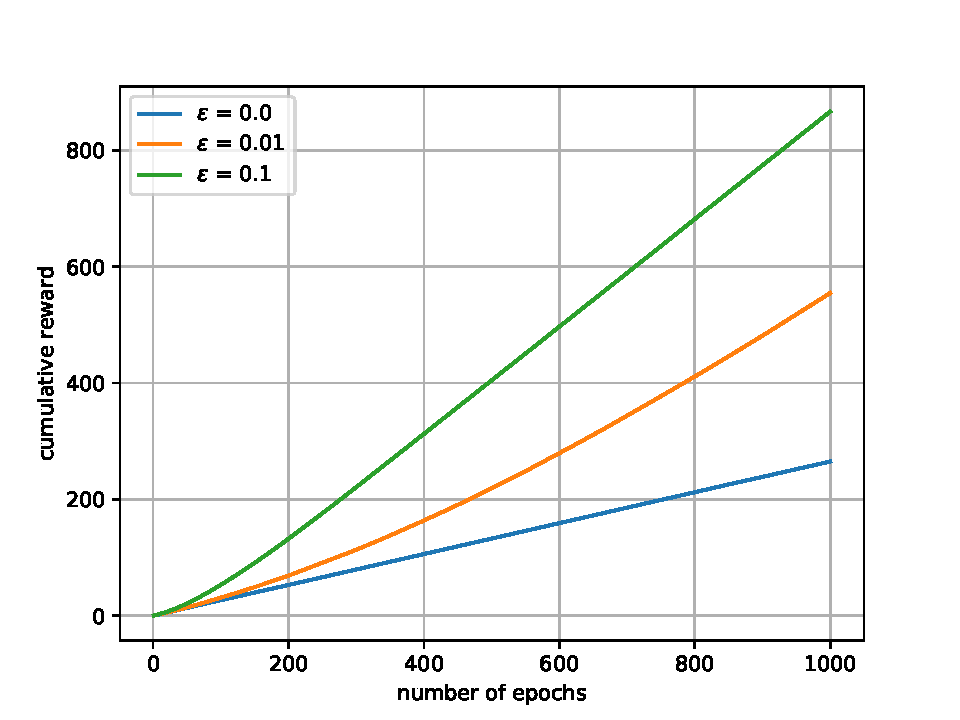
\includegraphics[width=\textwidth]{Report/sections/Figures/Figure4.pdf}
        \caption{Recompenses cumulés en fonction du nombre d'étape d'apprentissage}
    \end{subfigure}
    
    \caption{Performance des algorithmes Greedy et $\epsilon$-Greedy}
\end{figure}
\newpage
La figure 2 illustre une comparaison entre la méthode $Greedy$ et deux autres méthodes $\epsilon$-$Greedy$ ($\epsilon$=0.01 et $\epsilon$=0.1). On remarque que le regret cumulé et le nombre de récompenses augmentent avec le nombre de pas d'apprentissage, on peut observer également qu'au tout début, l'algorithme $Greedy$ s'améliore en apprentissage au même rythme que les deux autres algorithmes puis on voit une diminution en performance. En effet, la méthode gloutonne effectue uniquement de l'exploitation, autrement dit, elle se contente de choisir l'action la plus prometteuse à un instant donné sans explorer d'autres actions qui pourrait l'être davantage, les echantillonages initiaux qu'elle a effectué sont avérés être sous optimaux par la suite ce qui explique son déclin de performance.
La méthode $\epsilon$-$Greedy$ avec $\epsilon$=0.1 a exploré bien plus que la méthode $\epsilon$=0.01 ce qui explique que la plupart du temps elle identifie l'action optimale assez rapidement. La méthode $\epsilon$-$Greedy$ avec $\epsilon$=0.01 s'améliore en apprentissage plus lentement car elle exploite plus mais à un moment donnée, on est sensé observer un gain de performance de tel sorte qu'elle donne de meilleurs résultats que $\epsilon$-$Greedy$ avec $\epsilon$=0.1.
\newline
#TODO: il serait intéressant de changer la dispersion des valeurs des récompenses, il me semble que si elles sont trop dispersées c'est à dire avec une variance non négligeable, il nous faudra plus d'exploration pour trouver l'action optimale et dans ce cas $\epsilon$-$Greedy$ sera plus pérformante que Greedy. mais si on a une variance assez faible, l'algorithme Greedy sera plus performant car il trouvera l'action optimale rapidement et ne fera plus d'exploration. à faire : courbe de l'evolution du pourcentage de gain afin qu'on puisse mieux observer le raisonnement précédent
